\section{Introduction}\label{sec: intro}

The blockchain ecosystem has fragmented into dozens of independent Layer-1 and Layer-2 networks. As of 2024, over \$40 billion in total value locked (TVL) is distributed across chains such as Ethereum, Arbitrum, Optimism, Base, and Polygon~\cite{defillama}. Cross-chain bridges have emerged as the critical infrastructure enabling asset transfers between these networks, processing billions of dollars in daily volume.

However, bridging assets is neither cheap nor predictable. A user who wants to move \$500 of USDC from Ethereum to Optimism faces a complex decision: Across Protocol charges approximately \$3.33 in fees but completes in 27 seconds; Stargate V2 Bus amortizes gas across passengers for lower absolute costs but with 4-minute latency; CCTP offers trust-minimized USDC burns but takes 2.4 hours. No existing tool enables a user to compare these trade-offs in real time, let alone predict what fees will look like under different market conditions.

\subsection{Motivation}\label{sec: motivation}

The cost of cross-chain bridging is driven by multiple interacting factors that are difficult for end users to reason about:

\begin{enumerate}
    \item \textbf{Source-chain gas prices.} Initiating a bridge transaction requires an on-chain transaction on the source network. Ethereum mainnet gas costs can vary from 5 to 200+ gwei within a single day, causing source-side fees to fluctuate by orders of magnitude. Layer-2 networks (Arbitrum, Optimism, Base) reduce this to fractions of a cent, creating a \textbf{46.9$\times$ cost difference} driven purely by the user's choice of origin chain.

    \item \textbf{Destination-chain liquidity depth.} On liquidity-pool bridges (e.g., Stargate), the fee is a function of how much of the destination pool the transfer consumes. Larger transfers deplete more liquidity and incur higher spreads. On intent-based bridges (e.g., Across), independent relayers set competitive spreads, but these depend on the relayer's inventory risk and rebalancing costs.

    \item \textbf{Bridge protocol fee architecture.} Each protocol implements a fundamentally different fee model: Across uses input--output spreads set by relayer competition; Stargate Bus amortizes a fixed relay gas cost across co-passengers in a batch; CCIP charges a flat oracle-secured message fee; CCTP's cost is dominated by source-chain gas. These architectural differences mean the ``cheapest'' bridge varies by transfer amount, route, and time.

    \item \textbf{Real-time market conditions.} ETH price fluctuations affect USD-denominated gas costs. Network congestion creates temporal variations in both fees and latency. Token-specific liquidity depth introduces per-asset pricing differences: our analysis shows that illiquid tokens (e.g., POOL at 40.7 bps) cost nearly $10\times$ more than deep-liquidity assets (e.g., USDC at 4.1 bps).
\end{enumerate}

Without tools to understand, compare, and predict these costs, users make uninformed decisions---routinely overpaying for transfers when cheaper alternatives exist on competing protocols.

\subsection{Problem Statement \& Research Gap}\label{sec: problem}

\textbf{Problem Statement.} Users lack a unified tool to: (1)~compare live fees across multiple bridge protocols simultaneously, (2)~understand the structural decomposition of fees into gas, liquidity, and operator components, and (3)~predict future costs under varying market conditions using historical data.

\textbf{Research Gap.} Existing blockchain fee prediction work focuses primarily on single-chain gas price forecasting. LSTM networks with wavelet denoising have been proposed for Ethereum gas prediction~\cite{lstm_gas}. Gradient boosting methods (LightGBM, CatBoost) have been applied to gas forecasting~\cite{gbm_gas}. An empirical study on cross-chain transactions~\cite{empirical_cc} provides foundational cost decomposition but does not build predictive models. Work on AI-driven routing for cost optimization~\cite{ai_routing} explores embedding-based approaches but targets path selection rather than fee prediction.

On the tooling side, blockchain explorers such as LayerZero Scan, Wormhole Scan, and Across Explorer provide post-hoc transaction tracking but do not offer predictive fee models or cross-protocol comparisons. Individual bridge UIs display estimated fees within their own protocol, but these are not comparable across bridges, and none use machine learning for prediction.

To the best of our knowledge, no prior work has built a generalizable, cross-protocol fee prediction framework that (a) decomposes costs across architectural families, (b) trains per-bridge ML models on historical transaction data, and (c) serves predictions alongside real-time API quotes in a unified platform.

\subsection{Contributions}\label{sec: contributions}

This work makes the following contributions:

\begin{enumerate}
    \item \textbf{Multi-protocol dataset and ETL pipeline.} We designed and executed a data extraction pipeline using Dune Analytics SQL queries for historical gas prices, the Across Protocol deposits API for real filled transactions, the LiFi aggregator API for systematic cross-bridge quotes, Etherscan Gas Oracle for real-time gas data, and CoinGecko API for ETH/USD price enrichment. The resulting dataset spans five protocol configurations over eight months (May--December 2024), totalling 9{,}964 seed transactions augmented to 354{,}897 samples for the Across protocol via continuous live data collection.

    \item \textbf{Cost decomposition framework.} We decompose cross-chain bridge costs into their constituent components: base gas fees, liquidity-based spreads, and operator costs. We show that the liquidity spread ($r = 0.73$) is the dominant cost driver, far exceeding gas fees ($r = 0.16$). This reframes the bridge fee problem from a network congestion issue to a liquidity pricing problem.

    \item \textbf{Fee structure equity analysis.} We demonstrate structural cost inequity: relayer gas costs are roughly constant regardless of transfer size, so small transfers ($<$\$100) bear a disproportionate fee burden. We also document the 46.9$\times$ cost disparity between Ethereum and L2 source chains.

    \item \textbf{Per-bridge ML prediction models.} We trained per-bridge XGBoost and LightGBM models on 16--20 engineered features, with time-based 80/20 splits to prevent temporal leakage. Best results: $R^2 = 0.917$ on Across (354K samples), $R^2 = 0.465$ on Stargate OFT, $R^2 = 0.382$ on Stargate Bus. A median-based fallback handles CCIP (11 samples).

    \item \textbf{End-to-end deployed platform.} We built and deployed BridgeCompare: a FastAPI backend serving live bridge quotes from Across API (\texttt{app.across.to/api/suggested-fees}) and LiFi aggregator (\texttt{li.quest/v1/advanced/routes}), alongside ML predictions with confidence scores. The Next.js frontend provides real-time comparison with fee decomposition breakdowns. A continuous data pipeline appends every live quote to the training set for model retraining.
\end{enumerate}


\section{Background \& Related Work}\label{sec: background_rw}

\subsection{Cross-Chain Bridges}
Cross-chain bridges enable the transfer of digital assets between independent blockchain networks. As the blockchain ecosystem has fragmented across Layer-1 chains (Ethereum, Polygon) and Layer-2 rollups (Arbitrum, Optimism, Base), bridges have become critical infrastructure. The primary architectural families include:

\begin{itemize}
    \item \textbf{Lock-and-mint bridges}, which lock assets on the source chain and mint wrapped representations on the destination chain.
    \item \textbf{Burn-and-mint bridges} (e.g., CCTP), where native issuers burn tokens on the source and mint canonical tokens on the destination, avoiding wrapped token risk.
    \item \textbf{Liquidity pool bridges} (e.g., Stargate), which maintain pools on both chains and execute swaps, sharing gas costs through batching mechanisms.
    \item \textbf{Intent-based relayer bridges} (e.g., Across), where independent relayers front liquidity on the destination chain and are later reimbursed, with fees driven by input--output spreads.
    \item \textbf{Oracle-secured bridges} (e.g., CCIP), which use decentralized oracle networks to verify cross-chain messages.
\end{itemize}

\subsection{Cost Models}
Bridge costs are not a single fee but a composite of several components:
\begin{itemize}
    \item \textbf{Source-chain gas:} The cost of submitting the bridge transaction on the origin chain, driven by network congestion.
    \item \textbf{Destination-chain gas:} The cost of executing the delivery transaction on the destination chain, often paid by a relayer or protocol.
    \item \textbf{Liquidity spread:} The difference between the deposited amount and the received amount, reflecting the cost of consuming destination-chain liquidity.
    \item \textbf{Protocol fees:} Fixed or percentage-based fees charged by the bridge operator for the relay service.
\end{itemize}

\subsection{Related Work}
Existing blockchain transaction explorers such as LayerZero Scan and Wormhole Scan provide post-hoc transaction tracking but do not offer predictive fee models. Within individual bridge UIs, some protocols display estimated fees, but these are protocol-specific and not comparable across bridges.

Academic work on blockchain fee prediction has focused primarily on single-chain gas price forecasting. Models using LSTM networks with wavelet denoising~\cite{lstm_gas} have been proposed for Ethereum gas price prediction. Gradient boosting methods (LightGBM, CatBoost) have been applied to Ethereum gas forecasting~\cite{gbm_gas}. An empirical study on cross-chain transactions~\cite{empirical_cc} provides foundational cost decomposition but does not build predictive models. Work on AI-driven routing for cost optimization~\cite{ai_routing} explores embedding-based approaches but targets path selection rather than fee prediction.

To the best of our knowledge, no prior work has built a generalizable, cross-protocol fee prediction framework that combines historical ML models with live quote aggregation.

\section{Data Collection \& Methodology}\label{sec: data_collection}

\subsection{Bridge Selection}
We selected four production cross-chain bridge protocols that collectively cover the dominant architectural families in use today:

\begin{itemize}
    \item \textbf{Across:} An intent-based relayer bridge where independent relayers front liquidity on the destination chain and are reimbursed on the source chain. Fees are primarily driven by the input--output spread charged by the relayer.
    \item \textbf{Stargate V2 (Bus and OFT modes):} A LayerZero-based bridge with two operating modes. \textit{Bus mode} batches multiple user transactions into a single cross-chain message, amortizing gas costs across passengers. \textit{OFT (Omnichain Fungible Token) mode} sends each transfer individually.
    \item \textbf{CCIP (Chainlink Cross-Chain Interoperability Protocol):} An oracle-secured bridge primarily used for high-value institutional transfers, resulting in a much higher average transfer size.
    \item \textbf{CCTP (Circle Cross-Chain Transfer Protocol):} Circle's native USDC burn-and-mint bridge, offering a trust-minimized pathway for USDC transfers without wrapped tokens.
\end{itemize}

\subsection{Data Sources}
Our primary dataset (\texttt{all\_ccc\_sampled.csv}) contains 9{,}964 cross-chain transaction records sourced from on-chain data providers. Each record includes a set of common fields shared across all protocols (Table~\ref{tab:common_cols}) and a set of protocol-specific fields that capture each bridge's unique mechanics.

\begin{table}[t]
\centering
\small
\caption{Common columns across all bridge datasets.}
\label{tab:common_cols}
\begin{tabular}{lll}
\toprule
Field & Field & Field \\
\midrule
id & src\_blockchain & src\_blockchain\_type \\
src\_transaction\_hash & src\_from\_address & src\_to\_address \\
src\_fee & src\_fee\_usd & src\_timestamp \\
src\_contract\_address & src\_symbol & dst\_blockchain \\
dst\_blockchain\_type & dst\_transaction\_hash & dst\_from\_address \\
dst\_to\_address & dst\_fee & dst\_fee\_usd \\
dst\_timestamp & dst\_contract\_address & dst\_symbol \\
deposit\_id & depositor & recipient \\
adjusted\_src\_fee\_usd & adjusted\_dst\_fee\_usd & operator\_cost \\
user\_cost & latency & bridge \\
dune\_hourly\_gas\_gwei & eth\_price\_at\_src & \\
\bottomrule
\end{tabular}
\end{table}

Common columns include source and destination blockchain identifiers, transaction hashes, wallet addresses, raw fees in native tokens and USD equivalents, timestamps, token symbols, and derived cost variables (\texttt{user\_cost}, \texttt{operator\_cost}, \texttt{adjusted\_src\_fee\_usd}, \texttt{adjusted\_dst\_fee\_usd}, \texttt{latency}).

Protocol-specific fields capture bridge-unique concepts. For Across, these include \texttt{input\_amount}, \texttt{output\_amount}, \texttt{quote\_timestamp}, \texttt{fill\_type}, and \texttt{exclusivity\_deadline}. For Stargate Bus, they include batching-related fields such as \texttt{bus\_fare}, \texttt{bus\_fare\_usd}, \texttt{executor\_fee}, and \texttt{dvn\_fee}. CCIP and CCTP share a simpler schema with only \texttt{amount}, \texttt{amount\_usd}, and CCIP additionally including \texttt{fee\_token} fields.

\subsection{Data Processing}

Raw data were split into per-protocol subsets and cleaned using a uniform pipeline. The cleaning procedure applied the following rules:

\begin{enumerate}
    \item \textbf{Exact-duplicate removal.} Rows where all fields were identical were dropped.
    \item \textbf{Negative latency removal.} Rows with \texttt{latency} $< 0$ were removed, as these indicate clock-synchronization errors rather than valid transactions.
    \item \textbf{Negative fee removal.} Rows where \texttt{src\_fee\_usd}, \texttt{dst\_fee\_usd}, or \texttt{user\_cost} were strictly negative were removed, as negative fees represent calculation errors.
    \item \textbf{Extreme latency removal.} Rows with \texttt{latency} $\geq 31{,}536{,}000$ seconds (one year) were removed, as these correspond to permanently stuck or abandoned transactions.
\end{enumerate}

After cleaning, the five protocol subsets were saved as individual CSV files: \texttt{across\_cleaned.csv} (3{,}405 rows), \texttt{stargate\_bus\_cleaned.csv} (3{,}126 rows), \texttt{stargate\_oft\_cleaned.csv} (2{,}898 rows), \texttt{cctp\_cleaned.csv} (519 rows), and \texttt{ccip\_cleaned.csv} (12 rows).

\subsection{Feature Engineering}\label{sec:feature_eng}

From the cleaned per-protocol datasets, we engineered 16 features for model training. These features are grouped into four categories:

\begin{enumerate}
    \item \textbf{Financial features (3):} \texttt{amount\_usd}, \texttt{log\_amount} ($= \log(1 + \texttt{amount\_usd})$), and \texttt{amount\_x\_gas} ($= \texttt{amount\_usd} \times \texttt{dune\_hourly\_gas\_gwei}$). The log-transformed amount improves tree-based splits on the heavy-tailed transfer size distribution, while the interaction term captures the joint effect of transfer size and gas conditions.

    \item \textbf{Gas features (5):} \texttt{dune\_hourly\_gas\_gwei} (Ethereum gas price at transaction hour), \texttt{gas\_1h\_lag} (1-hour lag), \texttt{gas\_6h\_avg} (6-hour rolling mean), \texttt{gas\_24h\_avg} (24-hour rolling mean), and \texttt{gas\_volatility\_24h} (24-hour rolling standard deviation). Gas data were sourced from Dune Analytics hourly queries and Etherscan daily averages.

    \item \textbf{Market features (3):} \texttt{eth\_price\_at\_src}, \texttt{eth\_price\_change\_1h} (percentage change), and \texttt{eth\_price\_24h\_avg} (24-hour rolling mean), sourced from CoinGecko API.

    \item \textbf{Temporal and categorical features (5):} \texttt{hour\_of\_day}, \texttt{day\_of\_week}, \texttt{is\_weekend}, \texttt{month} (temporal); and \texttt{route} ($= \texttt{src\_blockchain} \to \texttt{dst\_blockchain}$) and \texttt{src\_symbol} (token identifier), both label-encoded. Additionally, cyclical encodings \texttt{hour\_sin} and \texttt{hour\_cos} were computed as $\sin(2\pi h / 24)$ and $\cos(2\pi h / 24)$ to capture the circular nature of time-of-day.
\end{enumerate}

Volume context was captured via \texttt{bridge\_hourly\_volume}, the count of transactions per bridge per hourly window.


\section{Exploratory Data Analysis}\label{sec: data_analysis}

We analyzed Across and Stargate protocols from May to December 2024. We computed both Pearson and Spearman correlation coefficients across all major numeric variables. Table~\ref{tab:dataset_stats} summarizes the five protocol subsets after cleaning.

\begin{table}[h]
\centering
\caption{Summary statistics by bridge protocol after data cleaning.}
\label{tab:dataset_stats}
\begin{tabular}{lrrrr}
\toprule
\textbf{Protocol} & \textbf{Rows} & \textbf{Avg.\ Latency (s)} & \textbf{Avg.\ Amount (USD)} \\
\midrule
CCIP         &    12 &    810.6 & \$28,167 \\
Across       & 3,405 &     26.9 &  \$1,746 \\
CCTP         &   519 &  8,553.4 & \$18,116 \\
Stargate Bus & 3,126 &    252.9 &    \$665 \\
Stargate OFT & 2,898 &    220.6 &  \$1,809 \\
\bottomrule
\end{tabular}
\end{table}

The strongest and most important finding is the relationship between the transfer amount (\texttt{amount\_usd}) and the total user cost. The Spearman coefficient of 0.68 shows a clear positive trend---larger transfers consistently cost more. However, this relationship is not driven by gas fees. When we decomposed user cost into its components, the liquidity spread showed a strong correlation with transfer size ($r = 0.73$), while the gas component showed a weak one ($r = 0.16$). This reframes the cost problem: the dominant cost of bridging is a liquidity fee proportional to pool consumption, not a network fee.

Figure~\ref{fig:feature_corr} presents the top feature correlations with user cost for each bridge protocol. The divergent correlation profiles across protocols confirm that each bridge's fee structure is driven by fundamentally different factors.

\begin{figure}[t]
\centering
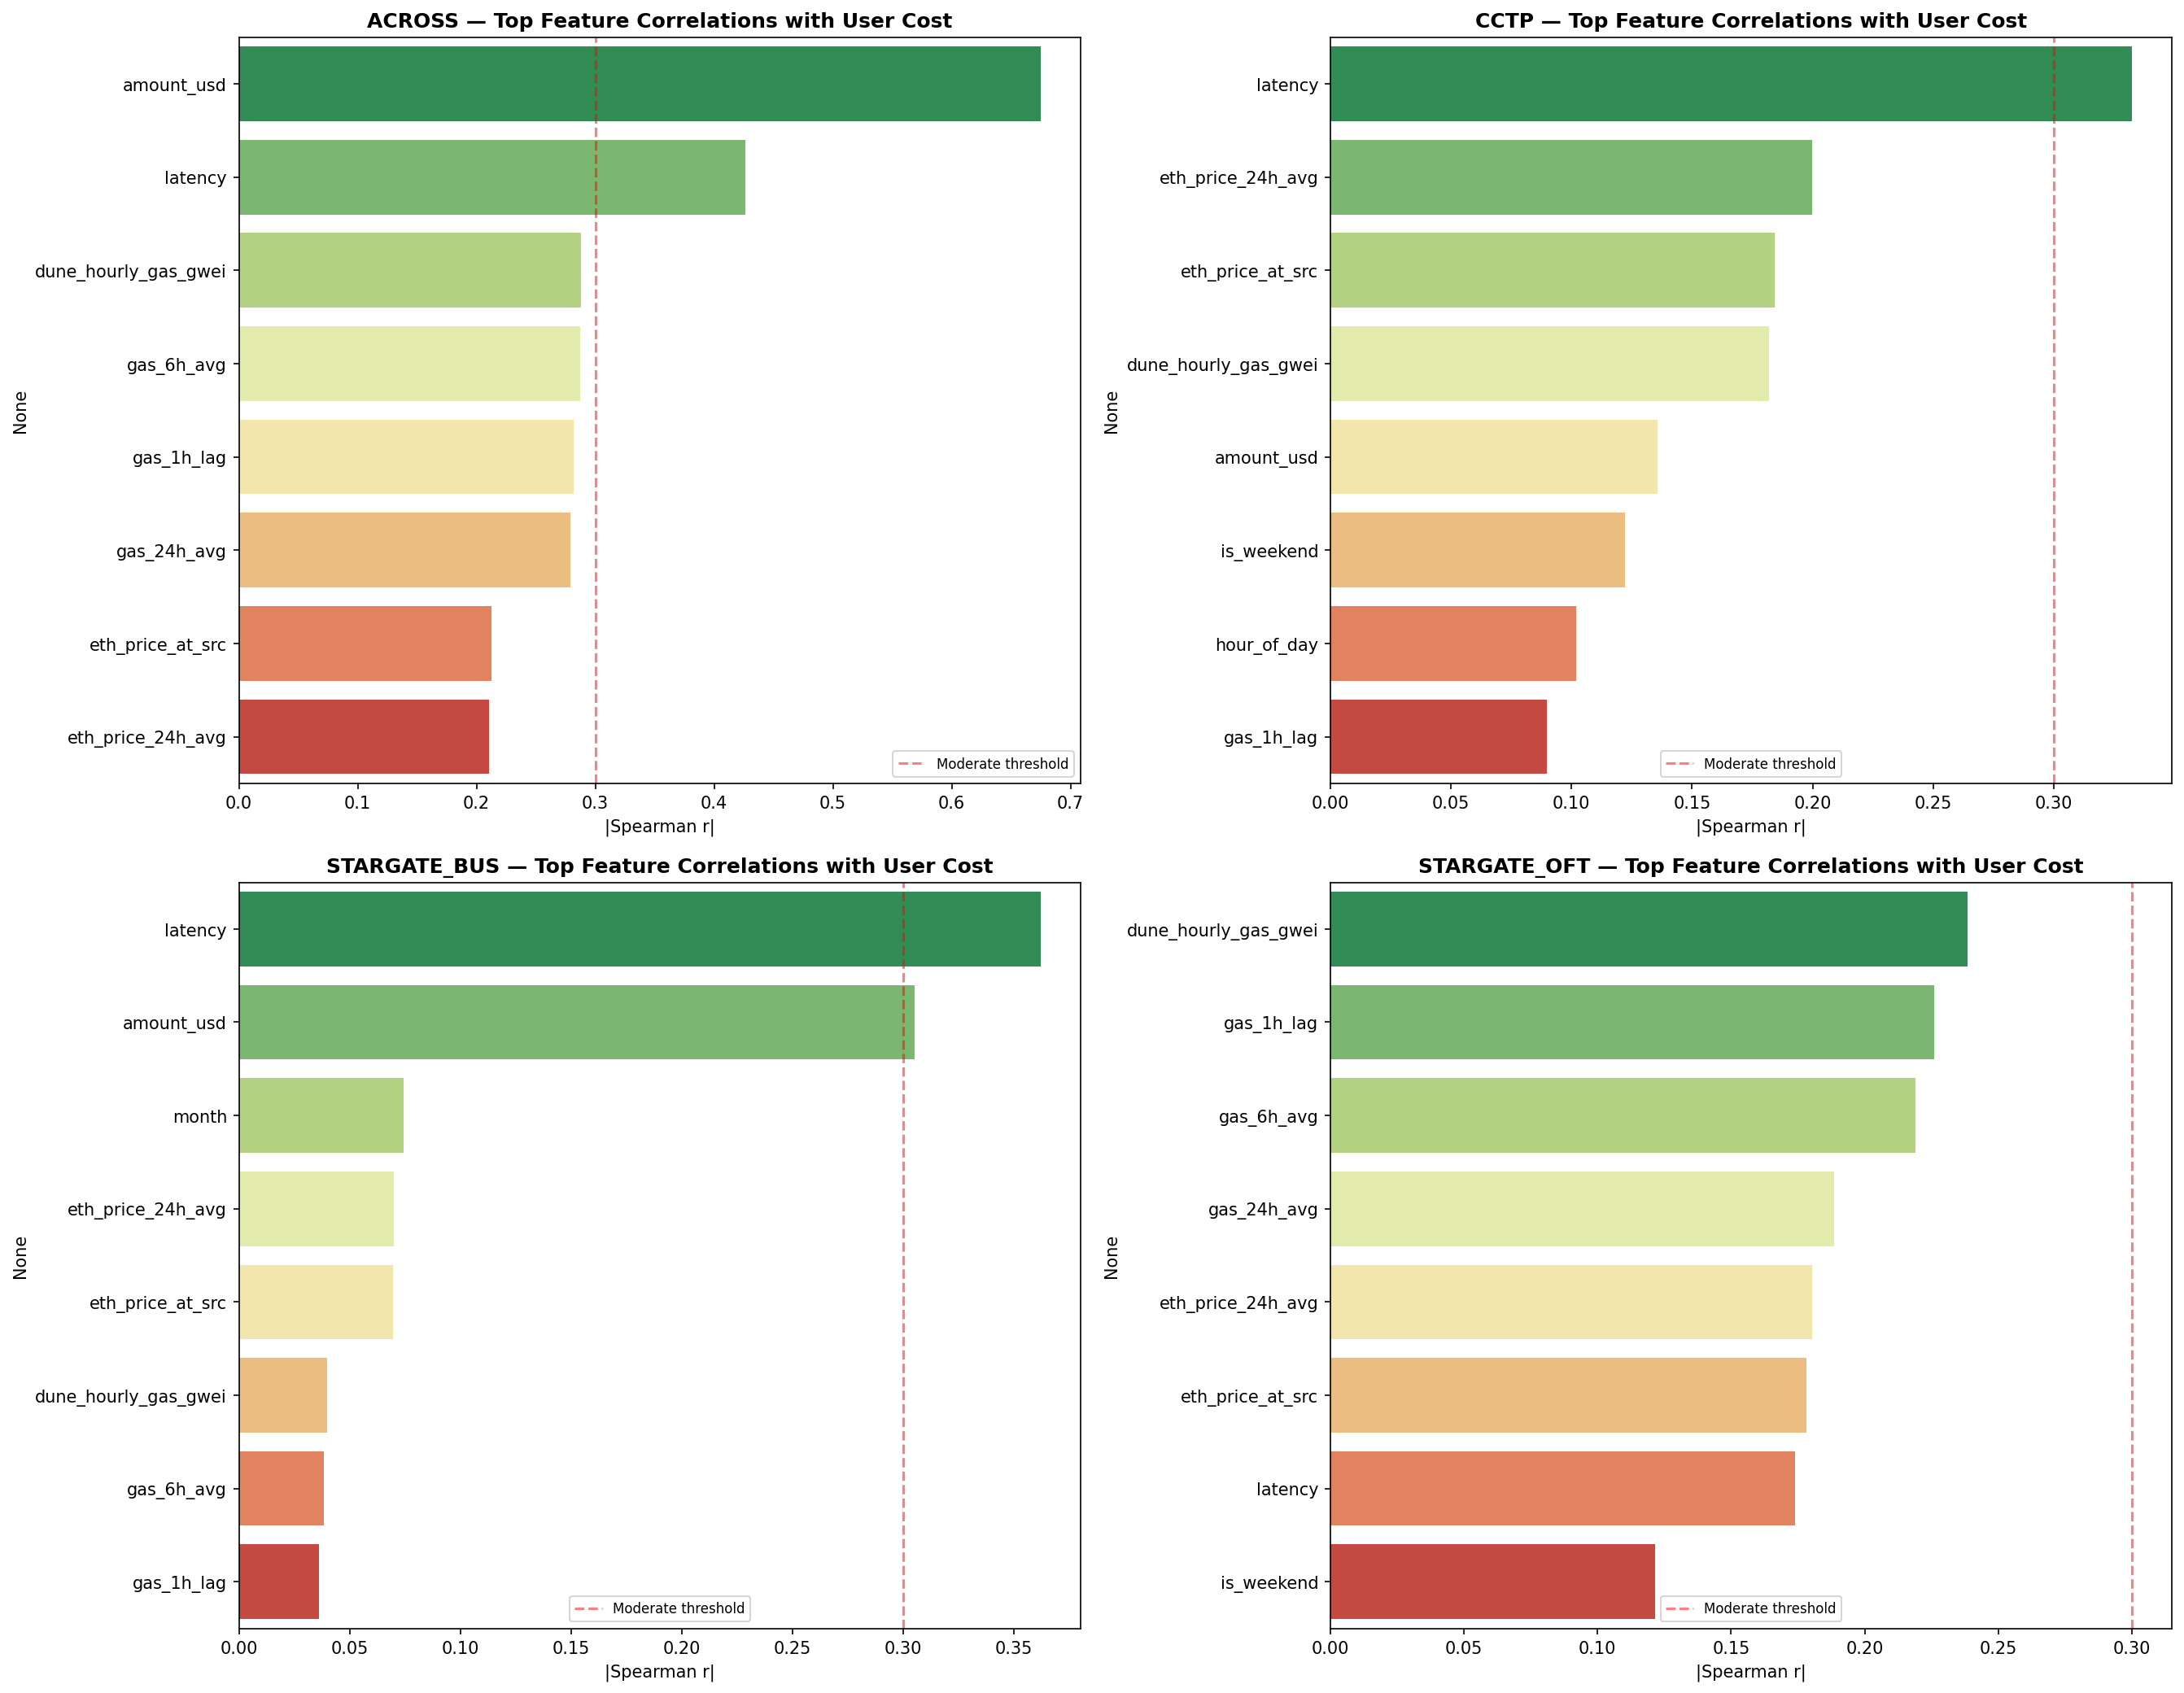
\includegraphics[width=\textwidth]{feature_correlation_per_bridge.png}
\caption{Top feature correlations with user cost by bridge protocol. Across is dominated by transfer amount ($|r| = 0.67$), while Stargate OFT depends on gas features ($|r| > 0.28$). The dashed red line marks the moderate correlation threshold ($|r| = 0.3$).}
\label{fig:feature_corr}
\end{figure}

Stargate V2 Bus mode has distinct behavioral characteristics arising from its batching architecture:

\begin{itemize}
    \item \textbf{Latency is independent of financial variables:} The correlation between execution latency and transfer size, gas price, or total fee is approximately $r \approx 0.06$---effectively zero. A large transfer and a small transfer experience the same delay if they are in the same batch.

    \item \textbf{Latency depends on user traffic:} The main factor determining wait time is how quickly other users submit transactions on the same route. The bus departs either when enough seats are filled or when a time limit is reached.

    \item \textbf{Cost sharing through batching:} Because gas costs are split among all passengers in a batch, individual users benefit from amortized fees. This makes per-transaction cost more stable and less sensitive to congestion spikes compared to the Across model.
\end{itemize}

\subsection{Across Protocol: Cost Drivers}

\subsubsection{Decomposing User Cost}

The strongest finding from the Across analysis is the relationship between transfer amount (\texttt{amount\_usd}) and total user cost. The Spearman coefficient of 0.68 shows a clear positive trend---larger transfers consistently cost more. When we decomposed \texttt{user\_cost} into its constituent parts, a more nuanced picture emerged:

\begin{table}[h]
\centering
\caption{Spearman correlation of user cost components with transfer amount (Across, $n = 3{,}411$).}
\label{tab:cost_decomp}
\begin{tabular}{lc}
\toprule
\textbf{Component} & \textbf{Spearman $r$ vs.\ \texttt{amount\_usd}} \\
\midrule
\texttt{user\_cost} (total)     & 0.6749 \\
Spread (input $-$ output)       & 0.7354 \\
Gas component                   & 0.1586 \\
\bottomrule
\end{tabular}
\end{table}

The liquidity spread---the difference between what the user deposits and what arrives at the destination---is the real cost driver ($r = 0.73$). The gas component is nearly independent of transfer size ($r = 0.16$). This finding is important because it reframes the cost problem: the dominant cost of using a relayer bridge is not a network fee but a liquidity fee, proportional to how much of the destination pool the transfer consumes.

Figure~\ref{fig:confounding} visualizes this decomposition. The top-left panel shows user cost increasing with transaction value, colored by ETH price to test for confounding. The top-right panel isolates the spread component, confirming the strong linear relationship. The bottom-left shows the gas component's independence from transfer size. The bottom-right provides ETH price context over the dataset period.

\begin{figure}[t]
\centering
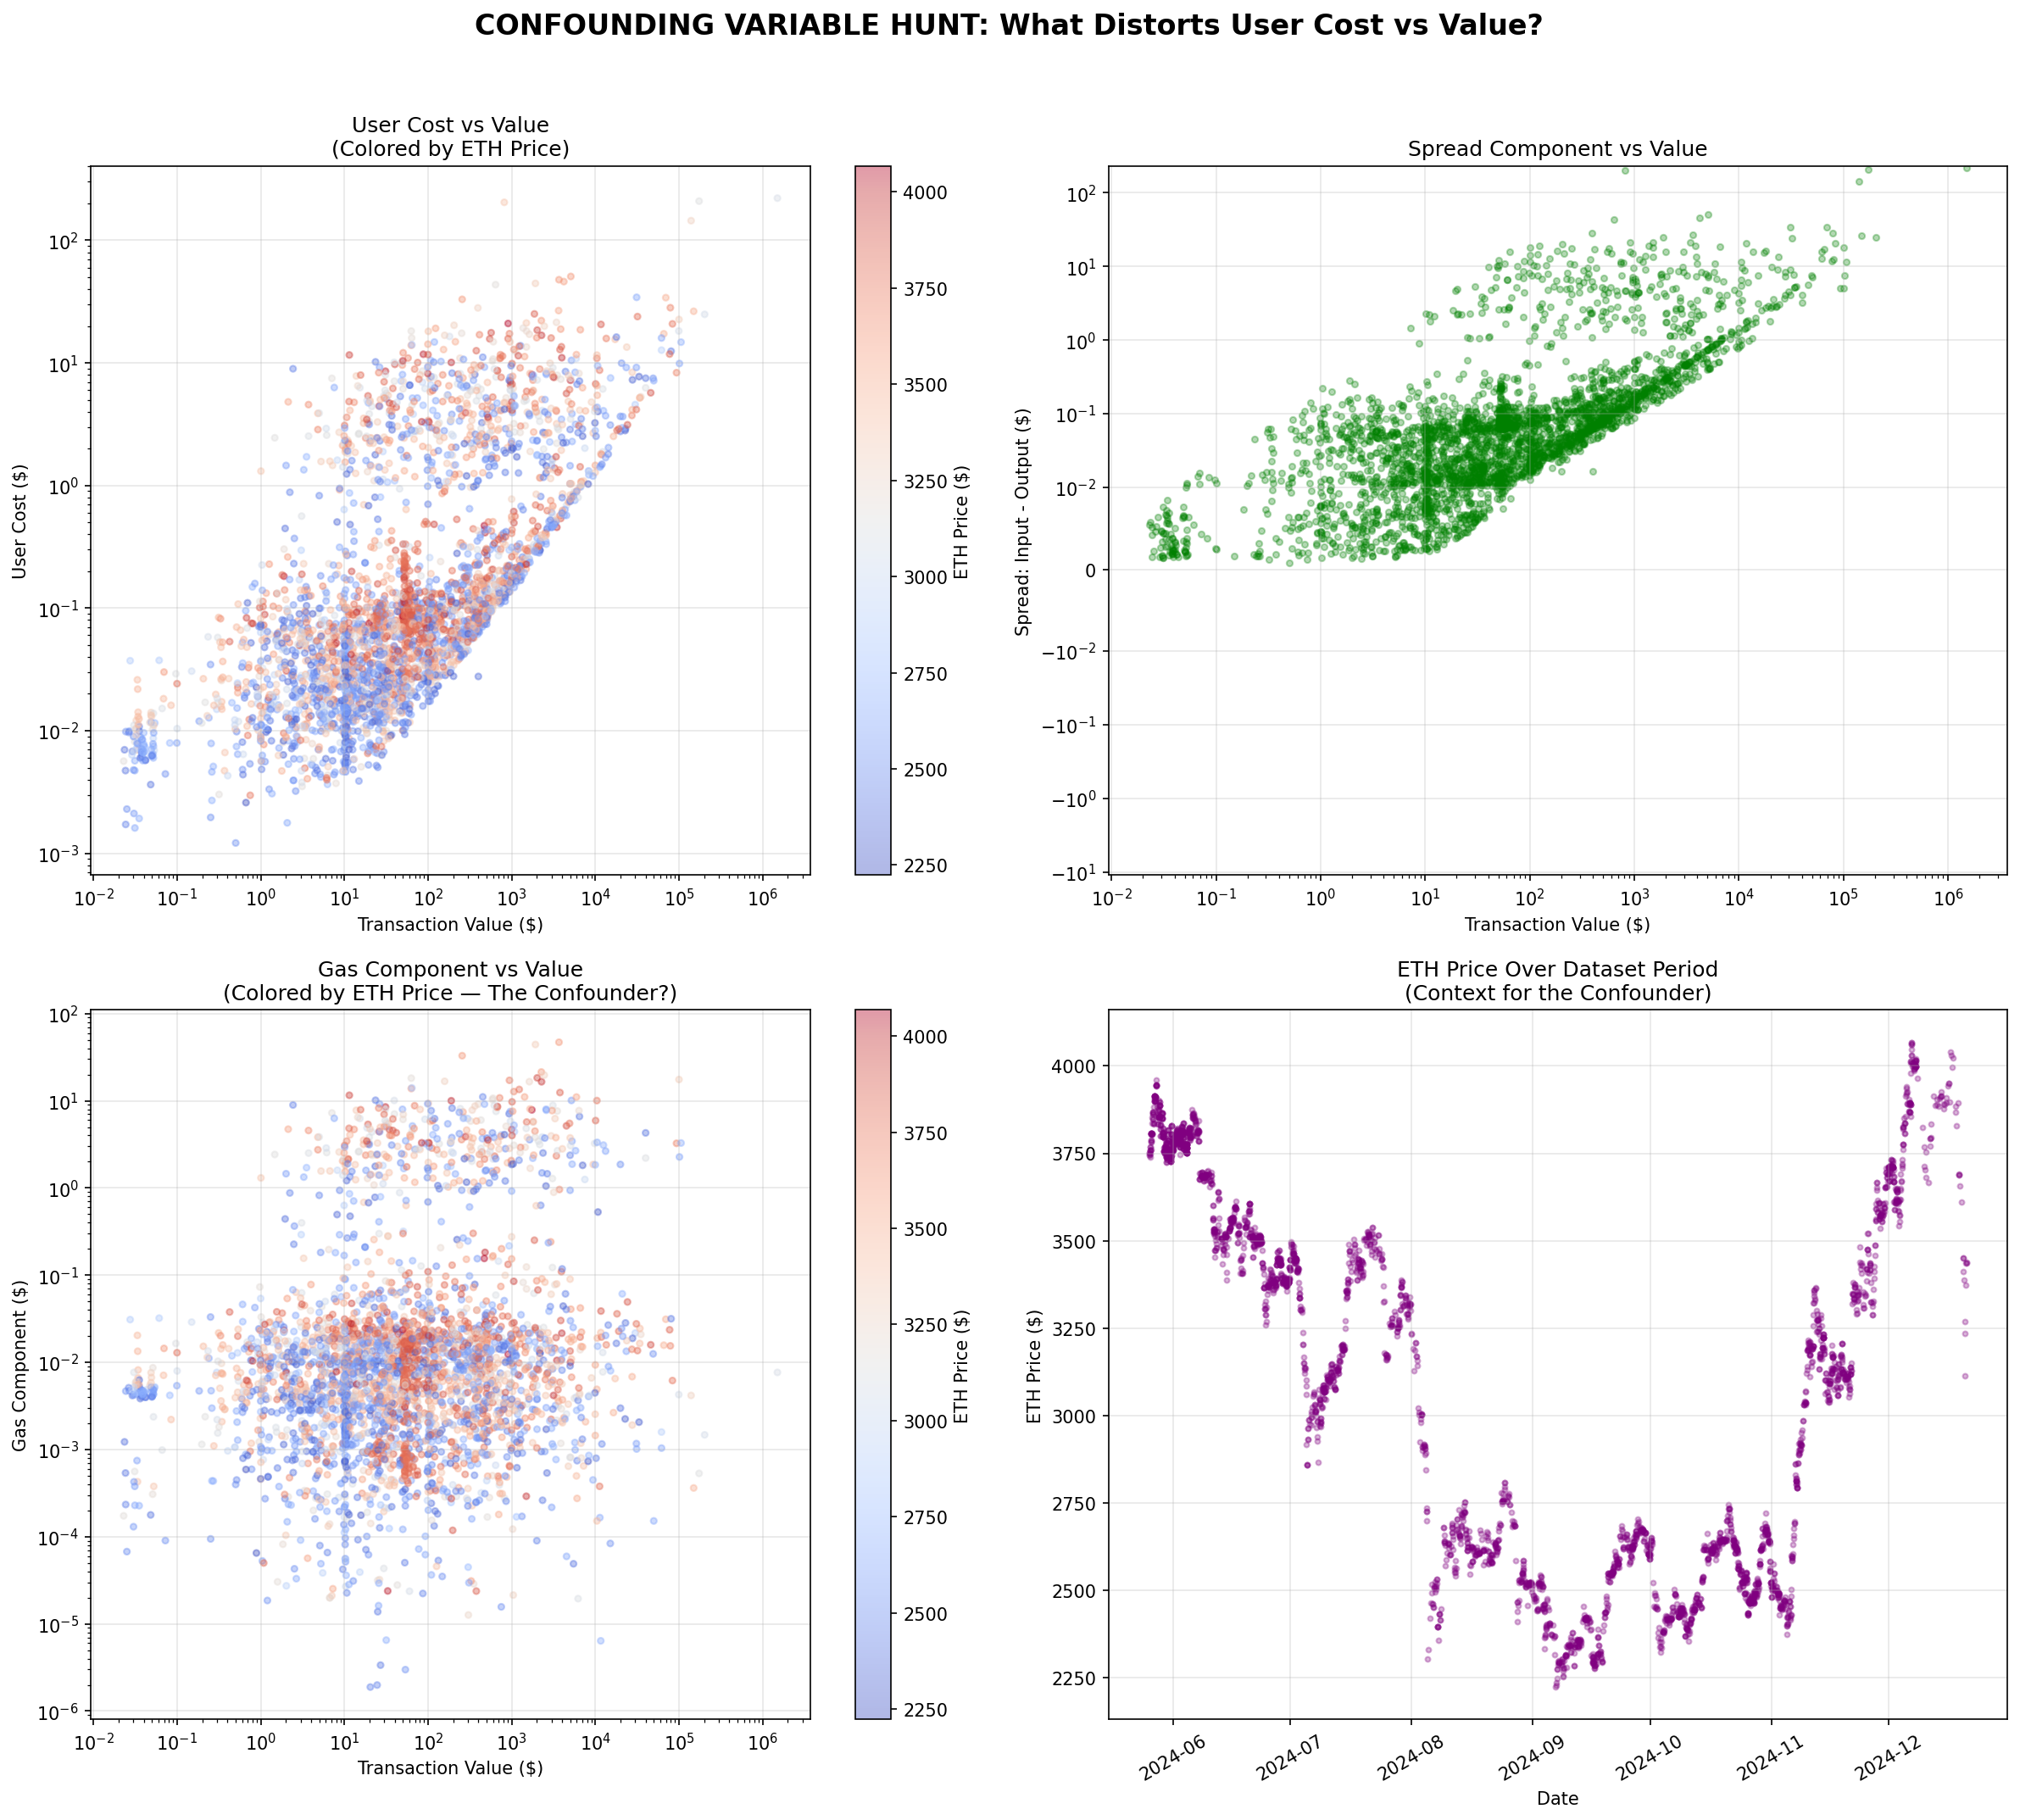
\includegraphics[width=\textwidth]{cleaned_split_data/confounding_variable_analysis.png}
\caption{Confounding variable analysis for Across. Top-left: User cost vs.\ transaction value (colored by ETH price). Top-right: Spread component vs.\ value, showing the dominant linear relationship. Bottom-left: Gas component vs.\ value, confirming independence. Bottom-right: ETH price over the dataset period.}
\label{fig:confounding}
\end{figure}

\subsubsection{Latency and Fee: No Incentive Effect}

We tested three competing hypotheses about whether fees influence transaction speed on Across:

\begin{itemize}
    \item \textbf{Hypothesis A (Incentive):} Higher fees attract relayers faster, reducing latency. Predicted: negative correlation.
    \item \textbf{Hypothesis B (Congestion):} High fees and high latency are both symptoms of network congestion. Predicted: positive correlation.
    \item \textbf{Hypothesis C (Automation):} Relayers are bots that fill anything profitable immediately, regardless of fee magnitude. Predicted: no correlation.
\end{itemize}

\begin{table}[h]
\centering
\caption{Correlation between latency and cost-related variables (Across, $n = 3{,}268$, filtered for latency $< 24$ hours).}
\label{tab:latency_corr}
\begin{tabular}{lcc}
\toprule
\textbf{Factor} & \textbf{Spearman $r$} & \textbf{Verdict} \\
\midrule
Total fee (\texttt{user\_cost})     & 0.4495 & Weak positive (congestion effect) \\
Network gas (Gwei)                  & 0.0826 & No impact \\
Transfer size (\texttt{amount\_usd}) & 0.3290 & Weak positive (congestion effect) \\
\midrule
Pearson $r$ (user cost vs.\ latency)  & 0.0959 & -- \\
Spearman $r$ (user cost vs.\ latency) & 0.2554 & -- \\
\bottomrule
\end{tabular}
\end{table}

The overall verdict supports Hypothesis C. For the vast majority of users, latency is constant at approximately 27 seconds. The weak positive Spearman correlation is driven by a small tail of transactions where general network congestion simultaneously raises gas prices (pushing up fees) and slows block inclusion (increasing latency). Relayers are automated systems that fill any profitable transaction immediately; the delays that do exist are an external network phenomenon, not a bridge-internal behavior.

The similar correlation magnitude on both the source side (\texttt{src\_fee\_usd} vs.\ latency: $r = 0.26$) and the destination side (\texttt{dst\_fee\_usd} vs.\ latency: $r = 0.21$) confirms that congestion-driven delays affect both chains equally---a further sign that network conditions, not bridge strategy, drive the effect.

Figure~\ref{fig:stargate_latency} visualizes the three latency hypotheses for Stargate. Hypothesis A (``Pay for Speed'') shows no correlation ($r = 0.06$) between fee and latency. Hypothesis B (``Gas Sensitivity'') shows weak negative correlation ($r = -0.07$). Hypothesis C (``Whale Neutrality'') confirms that large transfers experience the same latency as small ones ($r = 0.06$).

\begin{figure}[t]
\centering
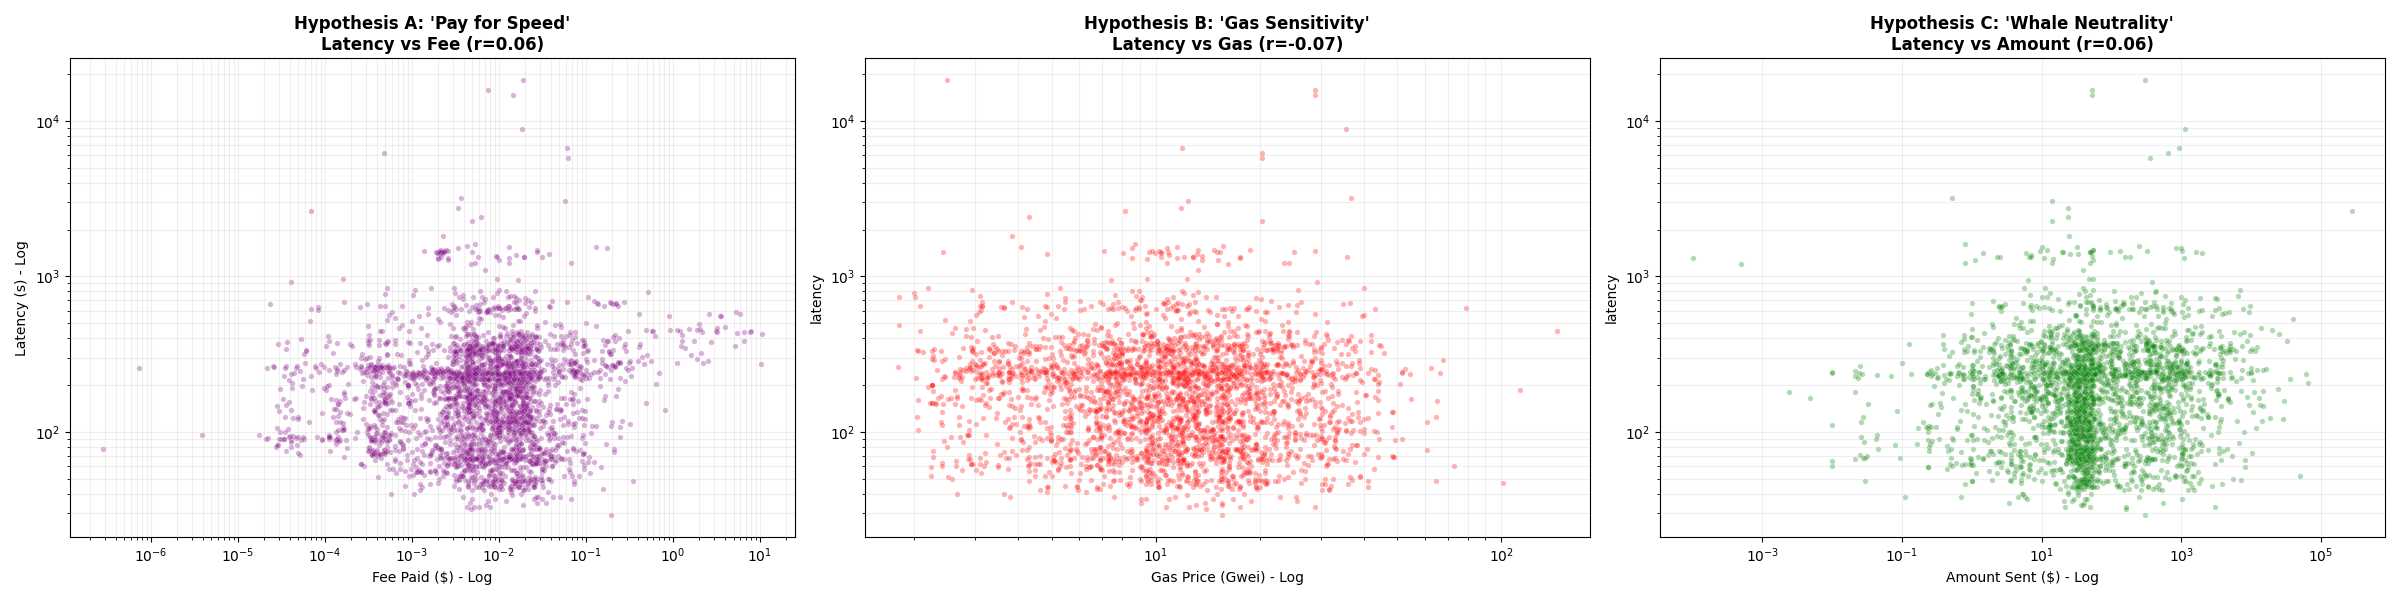
\includegraphics[width=\textwidth]{stargate_latency_analysis.png}
\caption{Stargate latency hypothesis testing. Left: Latency vs.\ fee paid ($r = 0.06$). Center: Latency vs.\ gas price ($r = -0.07$). Right: Latency vs.\ transfer amount ($r = 0.06$). All correlations are effectively zero, confirming that Stargate's batching architecture makes latency independent of financial variables.}
\label{fig:stargate_latency}
\end{figure}

\subsubsection{Source Chain as the Dominant Cost Factor}

A breakdown of median user cost by source blockchain reveals the single most actionable cost driver:

\begin{table}[h]
\centering
\caption{Median user cost by source blockchain (Across, $n = 2{,}618$).}
\label{tab:chain_cost}
\begin{tabular}{lc}
\toprule
\textbf{Source Chain} & \textbf{Median User Cost (USD)} \\
\midrule
Ethereum  & \$3.33 \\
Polygon   & \$0.11 \\
Linea     & \$0.09 \\
Base      & \$0.09 \\
Arbitrum  & \$0.09 \\
Scroll    & \$0.08 \\
Optimism  & \$0.07 \\
\bottomrule
\end{tabular}
\end{table}

Sending from Ethereum costs a median of \$3.33, compared to \$0.07 from Optimism---a factor of \textbf{46.9$\times$}. This finding dominates all other cost variables. The choice of source chain is far more impactful than any other user decision, including the choice of bridge protocol.

\subsubsection{Token Liquidity and Fee Rate Disparity}

Normalizing fees by transfer amount yields the fee rate in basis points (bps), where 1~bps = 0.01\%. This normalization exposes the cost barrier for illiquid tokens:

\begin{table}[h]
\centering
\caption{Median fee rate (bps) by token symbol (Across).}
\label{tab:token_fee_rate}
\begin{tabular}{lc}
\toprule
\textbf{Token} & \textbf{Median Fee Rate (bps)} \\
\midrule
POOL  & 40.7 \\
USDT  & 15.8 \\
WETH  & 10.3 \\
WBTC  &  9.2 \\
BAL   &  7.9 \\
DAI   &  5.3 \\
USDC  &  4.1 \\
\bottomrule
\end{tabular}
\end{table}

POOL tokens incur a fee rate nearly ten times higher than USDC. This disparity reflects liquidity depth: relayers demand a larger spread to absorb the inventory risk of holding and rebalancing illiquid tokens.

\subsubsection{Temporal Stability of the Amount--Cost Relationship}

To verify that the cost structure is stable over time, we computed the monthly Spearman correlation between \texttt{amount\_usd} and \texttt{user\_cost}:

\begin{table}[h]
\centering
\caption{Monthly Spearman correlation between transfer amount and user cost (Across).}
\label{tab:monthly_corr}
\begin{tabular}{lcc}
\toprule
\textbf{Month} & \textbf{Spearman $r$} & \textbf{$n$} \\
\midrule
May 2024      & 0.51 & 237 \\
June 2024     & 0.65 & 764 \\
July 2024     & 0.68 & 429 \\
August 2024   & 0.79 & 325 \\
September 2024 & 0.71 & 414 \\
October 2024  & 0.62 & 522 \\
November 2024 & 0.57 & 511 \\
December 2024 & 0.62 & 209 \\
\bottomrule
\end{tabular}
\end{table}

The correlation is consistently positive across all eight months (0.51--0.79), confirming that the amount--cost relationship is a stable structural feature of the Across protocol, not a transient market phenomenon.

Figure~\ref{fig:cost_evolution} shows the temporal evolution of Across cost metrics. The top panel displays cost efficiency (basis points) over time with a 7-day moving average, the middle panel shows the absolute cost distribution on a log scale with daily averages, and the bottom panel provides the Ethereum gas price context.

\begin{figure}[t]
\centering
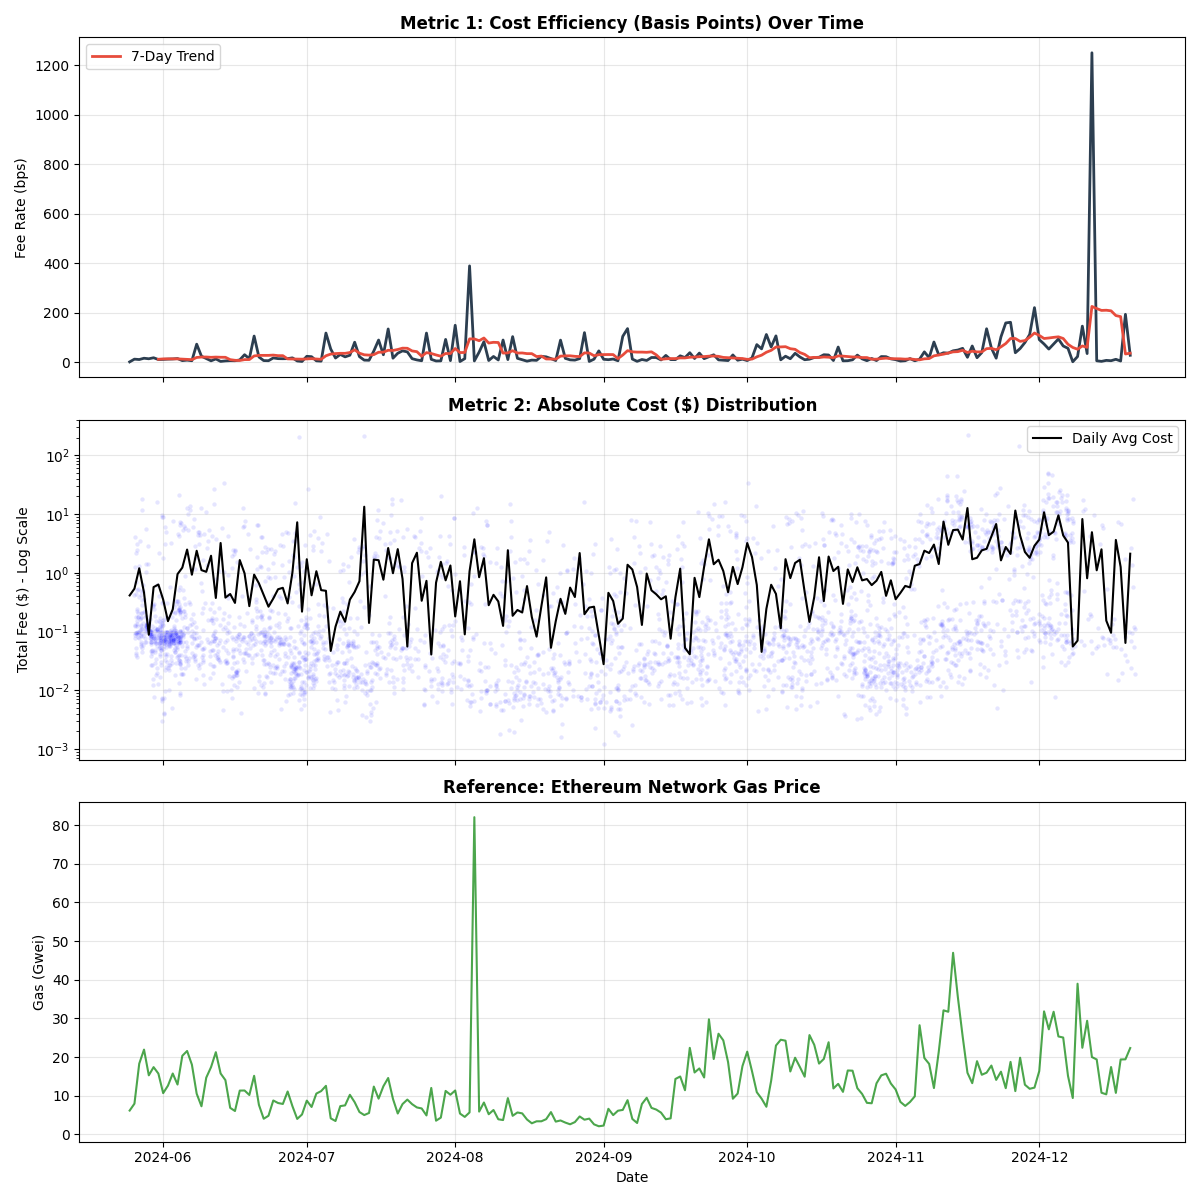
\includegraphics[width=0.85\textwidth]{cost_evolution_analysis.png}
\caption{Temporal evolution of Across bridge costs (May--December 2024). Top: Fee rate in basis points with 7-day trend line. Middle: Absolute cost distribution (log scale) with daily average. Bottom: Ethereum gas price in Gwei. The cost spikes in August and December coincide with gas price spikes, but the baseline fee rate remains stable.}
\label{fig:cost_evolution}
\end{figure}

\subsubsection{Confounding Variable Analysis}

To determine whether the relationship between \texttt{user\_cost} and \texttt{amount\_usd} is genuine, we conducted a partial correlation analysis controlling for each candidate confounder individually:

\begin{table}[h]
\centering
\caption{Partial correlation analysis: impact of confounders on the user cost--amount relationship (Across, $n = 3{,}407$).}
\label{tab:partial_corr}
\begin{tabular}{lccc}
\toprule
\textbf{Controlled Variable} & \textbf{Partial $r$} & \textbf{$\Delta$ from Raw} & \textbf{Impact} \\
\midrule
None (raw)                          & 0.6749 & --       & baseline \\
\texttt{latency}                    & 0.6296 & $-0.045$ & Moderate \\
\texttt{eth\_price\_at\_src}        & 0.6667 & $-0.008$ & Low \\
\texttt{src\_fee\_usd}              & 0.6841 & $+0.009$ & Low \\
\texttt{adjusted\_src\_fee\_usd}    & 0.6840 & $+0.009$ & Low \\
\texttt{dune\_hourly\_gas\_gwei}    & 0.6732 & $-0.002$ & Negligible \\
\bottomrule
\end{tabular}
\end{table}

The only confounder with any meaningful effect is \texttt{latency} ($\Delta = -0.045$), which mildly inflated the apparent relationship because it co-varies with both variables during congestion. Even after controlling for all confounders, the core relationship remains strong ($r \approx 0.63$--$0.69$), confirming it is a genuine structural property of the Across fee model.

Figure~\ref{fig:across_proof} provides visual evidence for two complementary findings. The left panel shows the ``ETH Tax'' effect: for retail users ($< \$1{,}000$), normalized cost (fee/amount) is weakly related to ETH price. The right panel shows the ``Liquidity Tax'' for whales ($> \$10{,}000$): higher fees correlate with slower fills, suggesting that large transfers consume more liquidity and experience delayed relayer activity.

\begin{figure}[t]
\centering
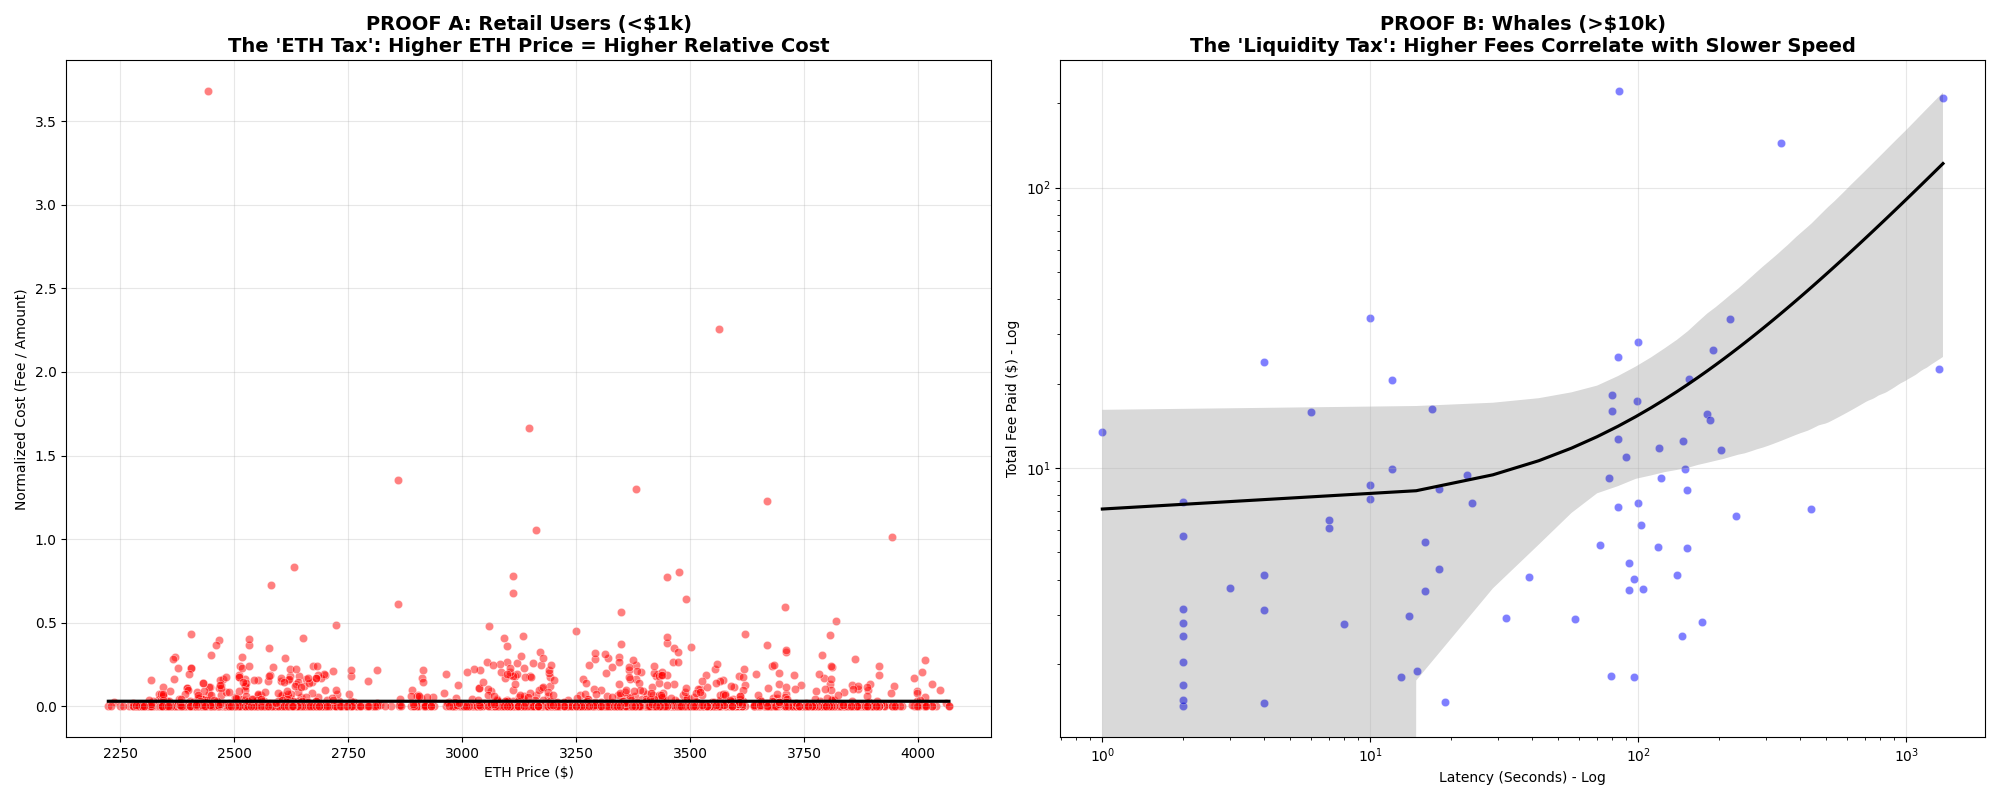
\includegraphics[width=\textwidth]{across_variable_proof.png}
\caption{Left: Normalized cost vs.\ ETH price for retail users ($< \$1{,}000$), showing the ``ETH Tax'' effect. Right: Total fee vs.\ latency for whale transfers ($> \$10{,}000$) with LOWESS trend line, demonstrating the ``Liquidity Tax'' where large transfers experience both higher fees and slower execution.}
\label{fig:across_proof}
\end{figure}

\subsection{Stargate V2: Architectural Differences and Cost Implications}

Stargate V2 Bus mode batches multiple cross-chain messages before relaying to the destination chain. This architectural choice has direct and measurable impacts on the data:

\begin{itemize}
    \item \textbf{Latency is independent of financial variables.} The correlation between execution latency and transfer size, gas price, or total fee is approximately $r \approx 0.06$---effectively zero. This contrasts sharply with Across, where congestion creates a weak but detectable cost--latency relationship.

    \item \textbf{Latency depends on user traffic.} The primary determinant of wait time is how quickly other users submit transactions on the same route. The bus departs either when enough seats are filled or when a time limit is reached, making latency a function of route popularity rather than network gas conditions.

    \item \textbf{Cost sharing through batching.} The fixed relay gas cost is amortized across all passengers in a batch, making the per-transaction gas component more stable and less sensitive to congestion spikes.

    \item \textbf{Src fee data unavailability.} All \texttt{src\_fee\_usd} values in the Stargate Bus dataset are \texttt{NaN}. This is a structural consequence of the bus model: the source-side fee is paid at the bus level, not at the individual transaction level, making per-user source fee attribution non-trivial from on-chain data alone.
\end{itemize}


\section{Cost Prediction Model}\label{sec: pred_model}

\subsection{Problem Formulation}

We frame cross-chain fee prediction as a per-bridge regression problem. Given a user's intended transfer parameters (source chain, destination chain, token, and amount) along with current market conditions (gas price, ETH price), the model predicts the total \texttt{user\_cost} in USD. Separate models are trained for each bridge protocol to capture their distinct fee architectures.

\subsection{Target Variable Transformation}

The distribution of \texttt{user\_cost} is heavily right-skewed across all protocols, with a small number of high-cost transactions inflating the tail. To stabilize variance and improve model performance, we apply the $\log(1+x)$ transformation to the target:
\begin{equation}
    y = \log_e(1 + \texttt{user\_cost})
\end{equation}
Predictions are mapped back to the original USD scale via the inverse transformation $\hat{y}_{\text{USD}} = \max(e^{\hat{y}} - 1, 0)$, with a floor at zero to prevent negative cost predictions.

\subsection{Model Architecture}

We employ a per-bridge ensemble evaluation strategy using gradient-boosted tree models:

\begin{itemize}
    \item \textbf{XGBoost} (primary model): 500 estimators, max depth 6, learning rate 0.05, subsample 0.8, \texttt{colsample\_bytree} 0.8, L1 regularization ($\alpha = 0.1$), L2 regularization ($\lambda = 1.0$), minimum child weight 3, with early stopping after 30 rounds of no improvement.
    \item \textbf{LightGBM} (challenger): Same hyperparameter configuration as XGBoost where applicable, with \texttt{verbose = -1} to suppress training output.
\end{itemize}

Both models are trained on each bridge's data, and the model with the higher $R^2$ on the held-out test set is selected as the winner for that bridge.

For \textbf{CCIP}, which has only 11 transactions in the dataset, we implement a \textbf{median-based fallback}: user cost is predicted by the median of historical transactions falling in the same transfer-size bucket ($[0, 100)$, $[100, 1{,}000)$, $[1{,}000, 10{,}000)$, $[10{,}000, 100{,}000)$, $[100{,}000, \infty)$ USD).

\subsection{Feature Set}

Each model uses up to 20 features drawn from the feature engineering pipeline described in Section~\ref{sec:feature_eng}. Table~\ref{tab:features} lists all features and their availability.

\begin{table}[h]
\centering
\small
\caption{Feature set for per-bridge prediction models. $\checkmark$ = available, (--) = missing for that bridge. The across model trained on 354K samples had only 11 features available.}
\label{tab:features}
\begin{tabular}{lcccc}
\toprule
\textbf{Feature} & \textbf{Across} & \textbf{CCTP} & \textbf{Stg. Bus} & \textbf{Stg. OFT} \\
\midrule
\texttt{amount\_usd}              & $\checkmark$ & $\checkmark$ & $\checkmark$ & $\checkmark$ \\
\texttt{log\_amount}              & $\checkmark$ & $\checkmark$ & $\checkmark$ & $\checkmark$ \\
\texttt{amount\_x\_gas}           & --            & $\checkmark$ & $\checkmark$ & $\checkmark$ \\
\texttt{dune\_hourly\_gas\_gwei}  & --            & $\checkmark$ & $\checkmark$ & $\checkmark$ \\
\texttt{gas\_1h\_lag}             & --            & $\checkmark$ & $\checkmark$ & $\checkmark$ \\
\texttt{gas\_6h\_avg}             & --            & $\checkmark$ & $\checkmark$ & $\checkmark$ \\
\texttt{gas\_24h\_avg}            & --            & $\checkmark$ & $\checkmark$ & $\checkmark$ \\
\texttt{gas\_volatility\_24h}     & --            & $\checkmark$ & $\checkmark$ & $\checkmark$ \\
\texttt{eth\_price\_at\_src}      & --            & $\checkmark$ & $\checkmark$ & $\checkmark$ \\
\texttt{eth\_price\_change\_1h}   & --            & $\checkmark$ & $\checkmark$ & $\checkmark$ \\
\texttt{eth\_price\_24h\_avg}     & --            & $\checkmark$ & $\checkmark$ & $\checkmark$ \\
\texttt{bridge\_hourly\_volume}   & $\checkmark$ & $\checkmark$ & $\checkmark$ & $\checkmark$ \\
\texttt{hour\_of\_day}            & $\checkmark$ & $\checkmark$ & $\checkmark$ & $\checkmark$ \\
\texttt{hour\_sin, hour\_cos}     & $\checkmark$ & $\checkmark$ & $\checkmark$ & $\checkmark$ \\
\texttt{day\_of\_week}            & $\checkmark$ & $\checkmark$ & $\checkmark$ & $\checkmark$ \\
\texttt{is\_weekend}              & $\checkmark$ & $\checkmark$ & $\checkmark$ & $\checkmark$ \\
\texttt{month}                    & $\checkmark$ & $\checkmark$ & $\checkmark$ & $\checkmark$ \\
\texttt{route\_enc}               & $\checkmark$ & $\checkmark$ & $\checkmark$ & $\checkmark$ \\
\texttt{src\_symbol\_enc}         & $\checkmark$ & $\checkmark$ & $\checkmark$ & $\checkmark$ \\
\bottomrule
\end{tabular}
\end{table}

\subsection{Training Procedure}

All models follow the same training procedure:

\begin{enumerate}
    \item \textbf{Filtering:} Rows where the target is null or non-positive are removed. Outliers beyond the 99th percentile of \texttt{user\_cost} are excluded to prevent extreme values from dominating the loss function.
    \item \textbf{Imputation:} Missing numeric feature values are filled with the column median.
    \item \textbf{Encoding:} Categorical features (\texttt{route}, \texttt{src\_symbol}) are label-encoded using scikit-learn's \texttt{LabelEncoder}. Encoders are persisted alongside the model so that unseen categories at inference time can be mapped to a default index.
    \item \textbf{Splitting:} Data is sorted chronologically by \texttt{src\_timestamp} and split 80/20. The earlier 80\% forms the training set; the later 20\% forms the test set. This \textbf{time-based split} prevents temporal leakage and simulates realistic deployment conditions where the model predicts future transactions.
    \item \textbf{Training:} XGBoost uses the test set as an early-stopping evaluation set, halting training after 30 rounds of no improvement in test loss.
    \item \textbf{Serialization:} The winning model, its encoders, and a metadata JSON file (containing features, training metrics, feature medians, feature importances, and confidence level) are serialized using \texttt{joblib} and stored in \texttt{backend/models/}.
\end{enumerate}

\subsection{Confidence Scoring}

Each model receives a confidence label based on its test-set $R^2$ and sample count:
\begin{equation}
\text{confidence} = \begin{cases}
\text{``low''} & \text{if } n < 50 \text{ or } R^2 < 0.4 \\
\text{``medium''} & \text{if } 0.4 \leq R^2 < 0.7 \\
\text{``high''} & \text{if } R^2 \geq 0.7
\end{cases}
\end{equation}


\section{System Architecture}\label{sec: system_arch}

Beyond the prediction model itself, we built an end-to-end platform that serves predictions alongside live bridge quotes through a web interface. Figure~\ref{fig:architecture} illustrates the full pipeline.

\subsection{Backend (FastAPI)}

The backend is implemented as a FastAPI application with the following endpoints:

\begin{table}[h]
\centering
\caption{API endpoints of the BridgeCompare backend.}
\label{tab:api_endpoints}
\begin{tabular}{llp{6.5cm}}
\toprule
\textbf{Method} & \textbf{Endpoint} & \textbf{Description} \\
\midrule
GET  & \texttt{/quotes} & Fetches live bridge quotes from Across API and LiFi aggregator, returns fee breakdowns and estimated times \\
GET  & \texttt{/predict} & Serves ML predictions for each bridge with confidence scores \\
GET  & \texttt{/eda} & Returns pre-computed EDA statistics (cost distributions, route analysis, hourly patterns) \\
GET  & \texttt{/data/stats} & Dataset statistics (row counts, bridge breakdown, time range) \\
GET  & \texttt{/model/status} & Model performance metrics ($R^2$, MAE, RMSE) per bridge \\
POST & \texttt{/model/retrain} & Triggers model retraining from accumulated live data \\
\bottomrule
\end{tabular}
\end{table}

\subsubsection{Live Quote Aggregation}

The \texttt{/quotes} endpoint aggregates real-time bridge pricing from two sources:

\begin{enumerate}
    \item \textbf{Across Protocol:} Direct API calls to \texttt{https://app.across.to/api/suggested-fees}, which returns a detailed fee breakdown including LP fee percentage, relayer gas cost, and capital fee. We normalize fees to USD using token decimals.

    \item \textbf{LiFi Aggregator:} API calls to \texttt{https://li.quest/v1/advanced/routes}, which routes through multiple protocols including CCTP, Stargate V2, CCIP, and deBridge. We parse each route to extract the bridge tool, compute the fee as the difference between input and output amounts, and separate gas costs from protocol fees.
\end{enumerate}

Quotes are cached for 30 seconds (\texttt{CACHE\_TTL\_SECONDS}) to reduce API load. Each quote is also persisted to \texttt{collected\_live\_data.csv} for future model retraining, along with real-time gas price (from Etherscan Gas Oracle API) and ETH price (from CoinGecko API).

\subsubsection{Prediction Service}

The \texttt{/predict} endpoint loads all trained models at startup via the \texttt{BridgePredictor} class. At inference time, it constructs a feature vector from the user's request parameters and current market data, runs predictions through all available bridge models, and returns each prediction with its confidence score, $R^2$, MAE, and training sample count.

For unseen routes or tokens at inference time, categorical encoders fall back to index 0 (the most common category). For missing numeric features, median values from the training set are substituted.

\subsection{Frontend (Next.js)}

The frontend is a Next.js~16 single-page application that provides:

\begin{itemize}
    \item \textbf{Transfer configuration:} Users select a source chain, destination chain, and transfer amount (in USDC). Supported chains include Ethereum, Arbitrum, Optimism, Base, and Polygon.
    \item \textbf{Live quote comparison:} Bridge quotes are displayed as cards sorted by fee, with ``Best Fee'' and ``Fastest'' badges. Each card shows the total fee, estimated transfer time, and an expandable fee breakdown (LP fee, relayer gas, capital fee, or protocol fee components).
    \item \textbf{ML prediction panel:} Alongside live quotes, model predictions are displayed with confidence badges (high/medium/low), $R^2$ scores, MAE error margins, and training data provenance (model vs.\ recent median).
\end{itemize}

\subsection{Continuous Data Pipeline}

The system implements a continuous learning loop:

\begin{enumerate}
    \item Every live quote fetched via \texttt{/quotes} is appended to \texttt{collected\_live\_data.csv} with the current gas price, ETH price, and temporal features.
    \item The \texttt{/model/retrain} endpoint triggers a full retraining run, loading both the original cleaned datasets and accumulated live data.
    \item Retrained models replace the existing ones in memory via hot-reload.
\end{enumerate}

\subsection{Deployment}

The backend is containerized via Docker (Python 3.11 slim, with models baked into the image during build) and deployed on Render. The frontend is deployed on Vercel. The Docker build process runs model training as part of the image build (\texttt{RUN python -m backend.train\_models}), ensuring that the deployed API always ships with up-to-date models.


\section{Results and Analysis}\label{sec: results_analysis}

\subsection{Model Performance}

Table~\ref{tab:model_results} presents the test-set performance of the trained models on their respective bridge datasets.

\begin{table}[h]
\centering
\caption{Test-set prediction performance per bridge. All metrics computed in original USD scale. The Across model was retrained on the expanded 354K dataset.}
\label{tab:model_results}
\begin{tabular}{lccccc}
\toprule
\textbf{Bridge} & \textbf{Model} & \textbf{$R^2$} & \textbf{MAE (\$)} & \textbf{RMSE (\$)} & \textbf{Confidence} \\
\midrule
Across       & XGBoost & 0.917 & 0.010 & 0.018 & High \\
Stargate OFT & XGBoost & 0.465 & 0.199 & 0.970 & Medium \\
Stargate Bus & XGBoost & 0.382 & 0.214 & 0.828 & Low \\
CCTP         & XGBoost & 0.025 & 3.554 & 10.869 & Low \\
CCIP         & Median  & --    & --    & --     & Low \\
\bottomrule
\end{tabular}
\end{table}

Figure~\ref{fig:actual_vs_predicted} visualizes the prediction quality for each bridge. Points closer to the red dashed diagonal ($y = x$) indicate more accurate predictions. Across shows tight clustering around the diagonal, while CCTP and Stargate Bus exhibit wider scatter.

\begin{figure}[t]
\centering
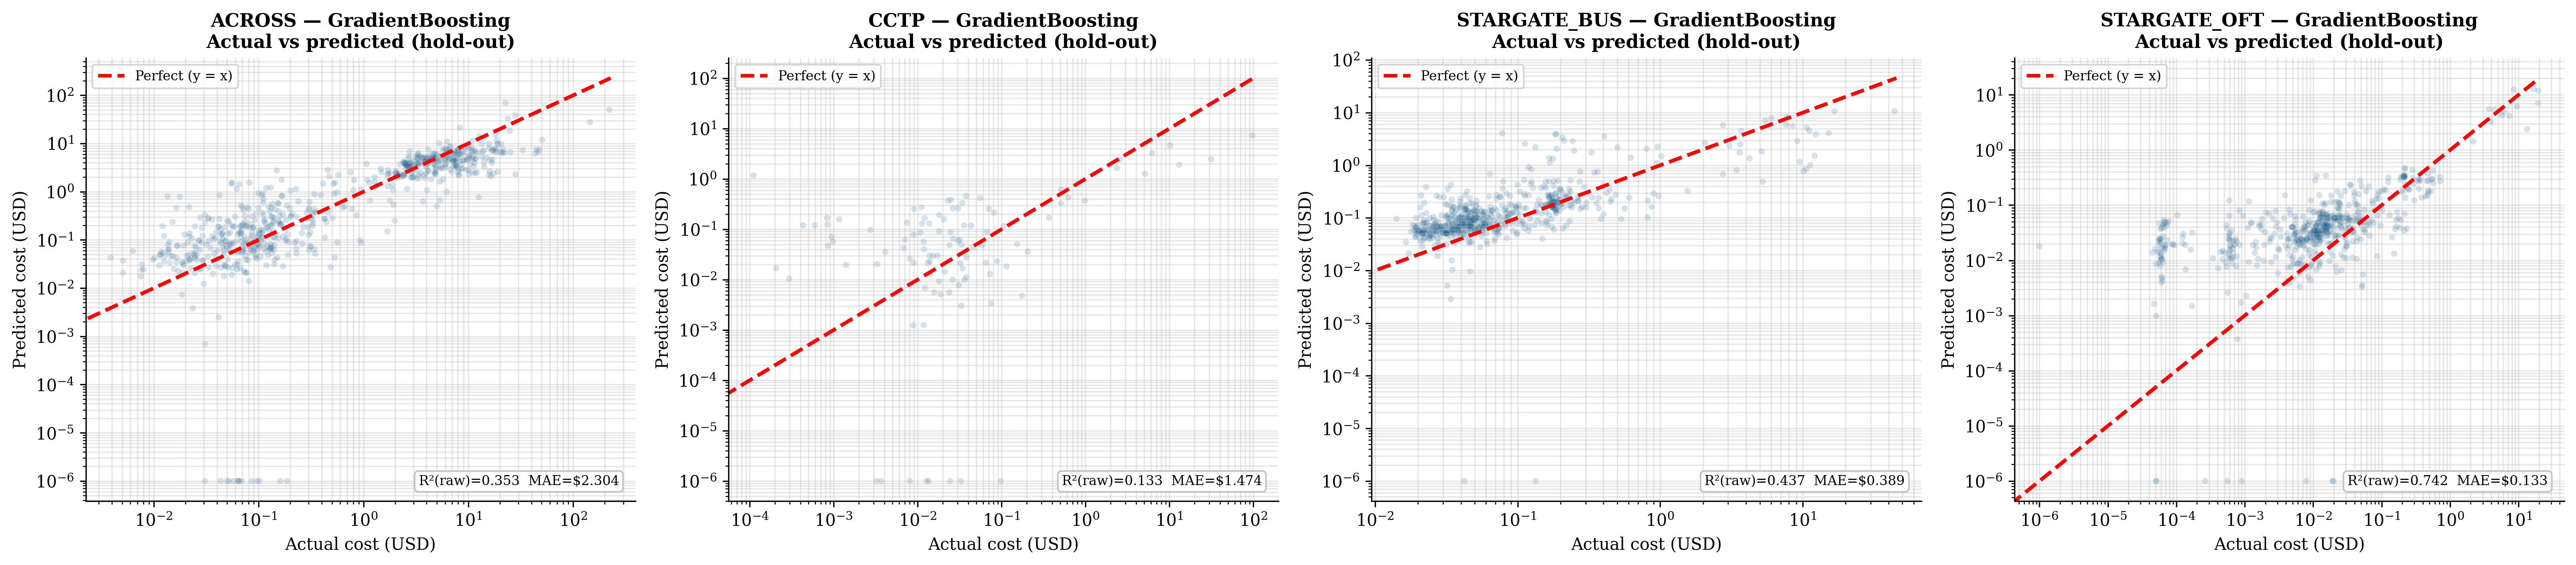
\includegraphics[width=\textwidth]{actual_vs_predicted_scatter.png}
\caption{Actual vs.\ predicted user cost (USD, log scale) for all four bridge models on held-out test sets. The red dashed line represents perfect prediction ($y = x$). Across shows tight agreement ($R^2 = 0.353$ in raw scale); Stargate OFT achieves reasonable performance ($R^2 = 0.742$); Stargate Bus and CCTP show higher dispersion.}
\label{fig:actual_vs_predicted}
\end{figure}

\subsubsection{Across Protocol ($R^2 = 0.917$)}

The Across model achieves the strongest performance, with an $R^2$ of 0.917 and an MAE of just \$0.01. This success is attributable to two factors: (1) the large training set (354{,}897 samples, obtained from an expanded dataset), and (2) the strong structural relationship between transfer amount and user cost, which the model captures via the \texttt{amount\_usd} and \texttt{log\_amount} features. Feature importance analysis (Table~\ref{tab:across_fi}) confirms that these two features account for 88\% of the model's total importance weight.

\begin{table}[h]
\centering
\caption{XGBoost feature importance for Across ($n = 354{,}897$). Top 5 features shown.}
\label{tab:across_fi}
\begin{tabular}{lc}
\toprule
\textbf{Feature} & \textbf{Importance} \\
\midrule
\texttt{log\_amount}          & 0.447 \\
\texttt{amount\_usd}          & 0.433 \\
\texttt{src\_symbol\_enc}     & 0.052 \\
\texttt{route\_enc}           & 0.012 \\
\texttt{hour\_sin}            & 0.011 \\
\bottomrule
\end{tabular}
\end{table}

The dominance of amount features is consistent with the EDA finding that the liquidity spread ($r = 0.73$) drives the cost---and the model has learned this structural relationship.

Figure~\ref{fig:feature_importance} presents the full feature importance profiles for all four bridge models. The contrasting importance distributions across bridges confirm that each protocol's fee structure is governed by different underlying factors.

\begin{figure}[t]
\centering
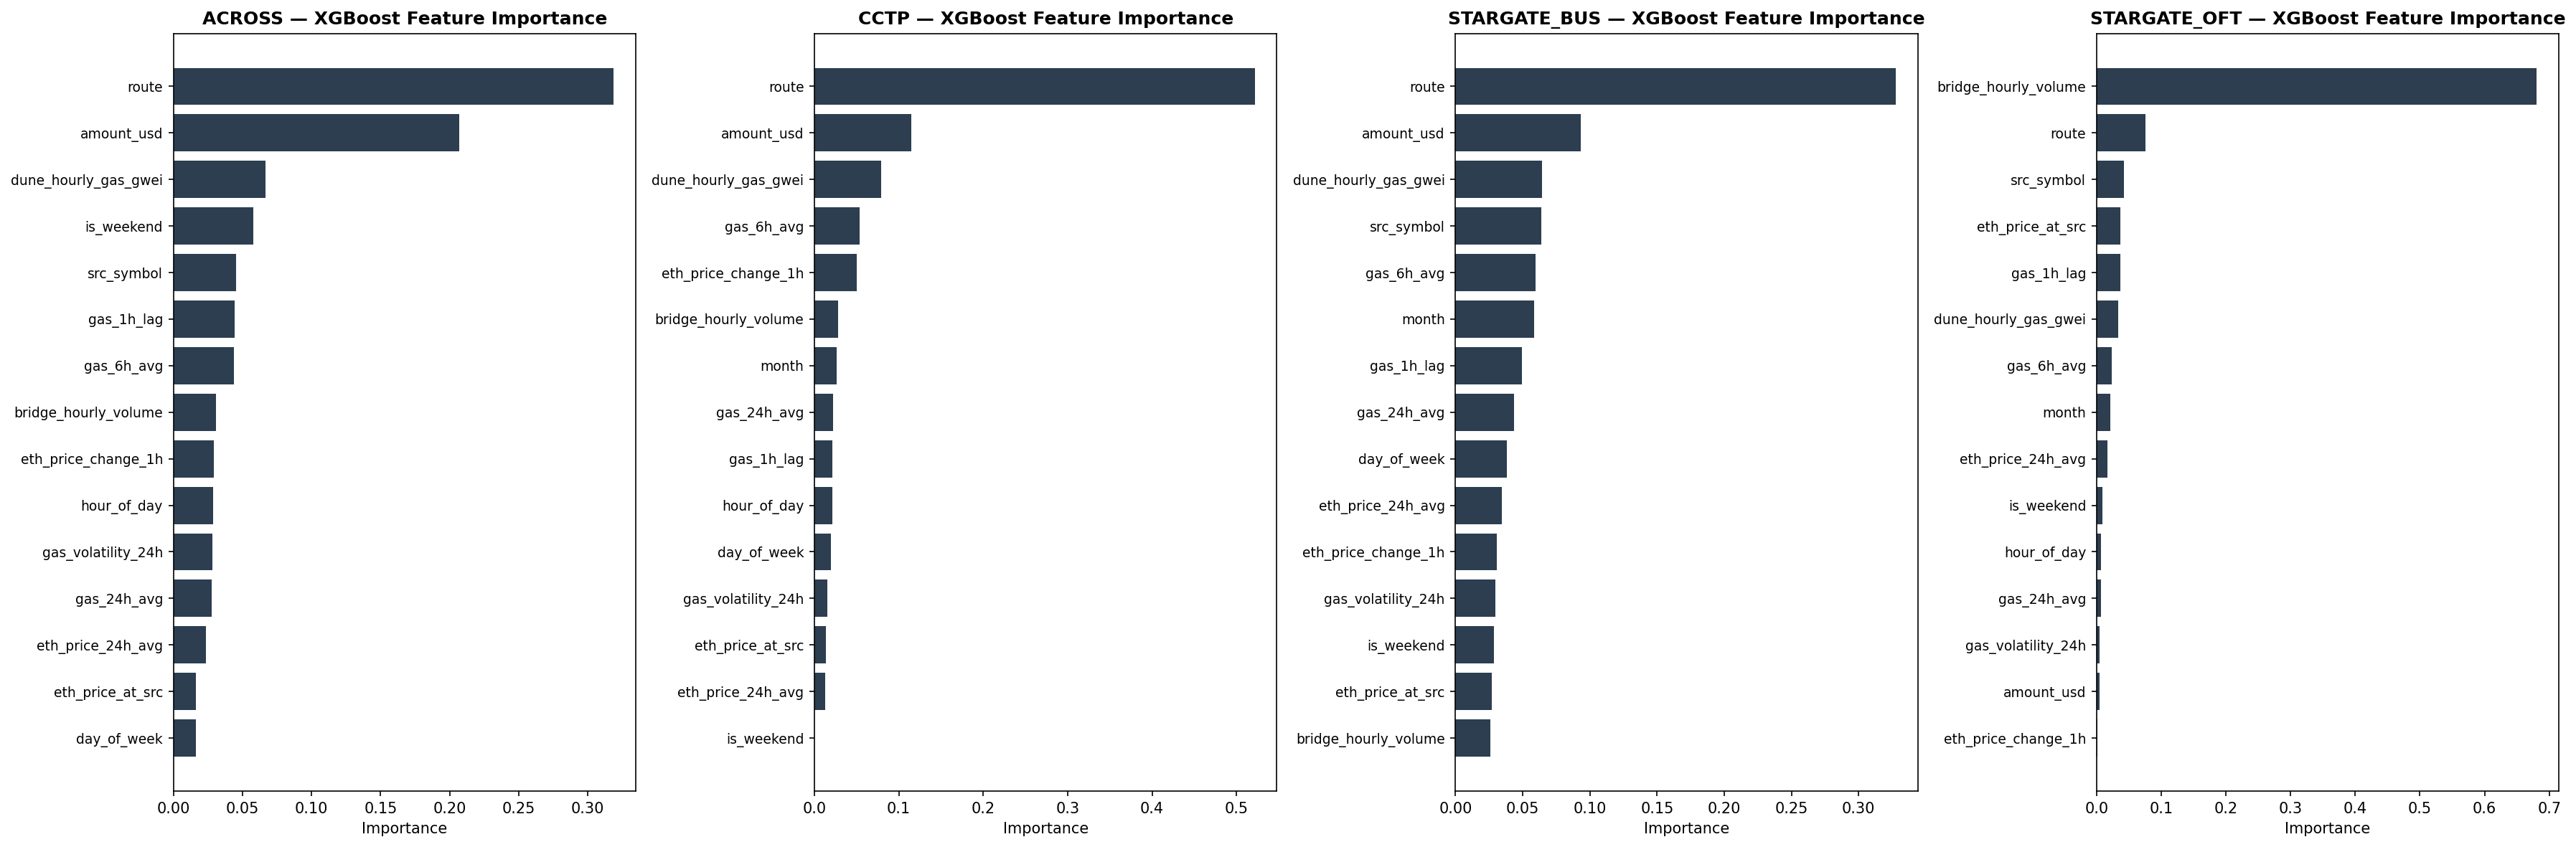
\includegraphics[width=\textwidth]{feature_importance_xgboost.png}
\caption{XGBoost feature importance across all four bridge models. Across is dominated by route and transfer amount; CCTP by route; Stargate Bus by route and amount; Stargate OFT by bridge hourly volume and route. These profiles align with each protocol's architectural fee mechanism.}
\label{fig:feature_importance}
\end{figure}

\subsubsection{Stargate OFT ($R^2 = 0.465$)}

The Stargate OFT model achieves moderate performance with an MAE of \$0.20. The most important feature is \texttt{bridge\_hourly\_volume} (importance = 0.478), reflecting how Stargate OFT fees depend heavily on how much concurrent traffic is using the same route. This is consistent with the liquidity pool design where each transfer's cost is influenced by the state of the shared pool.

\subsubsection{Stargate Bus ($R^2 = 0.382$)}

Stargate Bus has the weakest ML performance among protocols with sufficient data. This is a direct consequence of its batching architecture: individual transaction costs depend on the number of co-passengers in a batch, a variable that is not observable at prediction time. The most important feature is \texttt{route\_enc} (importance = 0.324), reflecting route-specific batching behavior. The model's inability to predict batch composition at inference time fundamentally limits its accuracy.

\subsubsection{CCTP ($R^2 = 0.025$)}

The CCTP model performs poorly, barely exceeding a constant baseline. With only 561 training samples and high variance in transfer sizes (\$150 median but up to \$18{,}116 average), the model lacks sufficient data to capture fee patterns. Additionally, CCTP's burn-and-mint mechanism produces a fee structure that is harder to predict from external features alone, as the primary fee is the source-chain gas cost which varies with network conditions. The highest-importance feature is \texttt{route\_enc} (0.399), suggesting significant route-level fee heterogeneity that the model cannot adequately capture with limited data.

\subsubsection{CCIP (Median Fallback)}

With only 11 transactions, CCIP is handled via a median-cost lookup stratified by transfer-size bucket. The median cost is \$1.08, but with a standard deviation of \$5.00, indicating high variability even within the small sample.

Figure~\ref{fig:error_dist} shows the prediction error distributions in log-space for each bridge. Across and Stargate Bus show error distributions tightly centered around zero, while CCTP exhibits a longer positive tail, reflecting systematic under-prediction on high-cost transactions.

\begin{figure}[t]
\centering
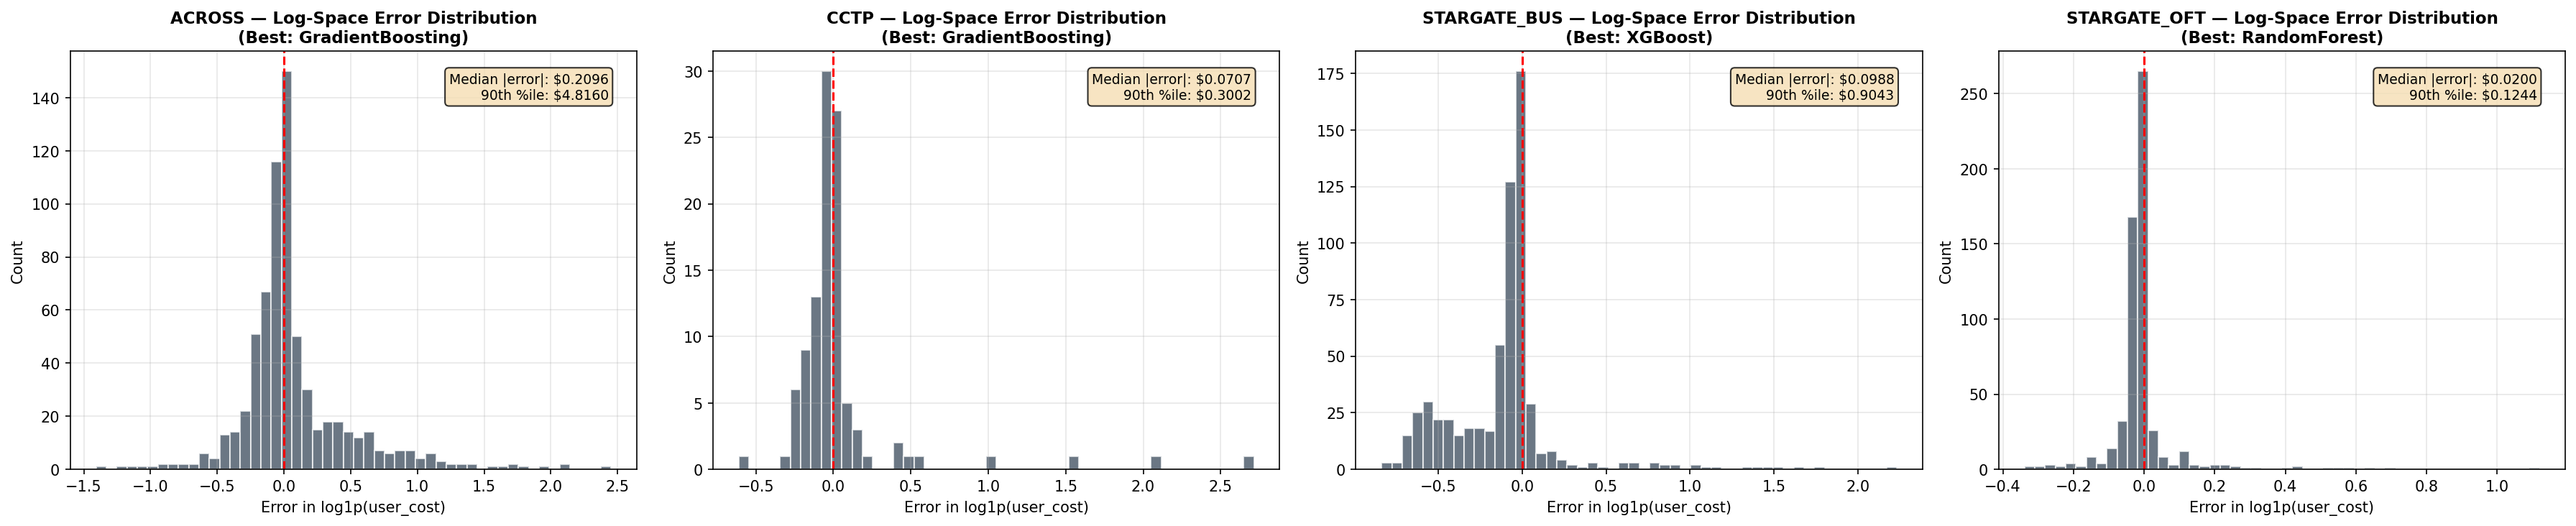
\includegraphics[width=\textwidth]{prediction_error_distribution.png}
\caption{Log-space prediction error distributions for each bridge model. The red dashed line marks zero error. Across: median error \$0.21, 90th percentile \$4.82. Stargate Bus: median \$0.10, 90th \$0.90. Stargate OFT: median \$0.02, 90th \$0.12. CCTP: median \$0.07, 90th \$0.30.}
\label{fig:error_dist}
\end{figure}

\subsection{Cross-Protocol Comparison}

Table~\ref{tab:cross_protocol} compares the protocols across key operational dimensions.

\begin{table}[h]
\centering
\caption{Cross-protocol comparison. Speed rank: 1 = fastest.}
\label{tab:cross_protocol}
\begin{tabular}{lcccc}
\toprule
\textbf{Protocol} & \textbf{Avg.\ Latency} & \textbf{Speed Rank} & \textbf{Avg.\ Transfer} & \textbf{Use Case} \\
\midrule
Across       &     27s & 1 &  \$1,746 & Retail, fast \\
Stargate OFT &  3.7 min & 3 &  \$1,809 & Medium-value \\
Stargate Bus &  4.2 min & 4 &    \$665 & Small-value, cost-shared \\
CCIP         & 13.5 min & 5 & \$28,167 & Institutional, high-value \\
CCTP         &  2.4 hr  & 2$^\ast$ & \$18,116 & High-value USDC \\
\bottomrule
\end{tabular}
\end{table}
\footnotesize{$^\ast$ CCTP standard latency is $\sim$2.4 hours; the ``fast'' variant via Celer achieves $\sim$2 minutes.}

\normalsize

\noindent \textbf{No single bridge dominates across all use cases.} Across is fastest and cheapest for retail-size L2$\to$L2 transfers. Stargate Bus provides the cheapest option for small transfers via cost amortization. CCTP is the most trust-minimized for USDC transfers. CCIP serves institutional use cases where oracle-level security justifies higher latency.


\section{Discussion}\label{sec: discussion}

\subsection{Key Findings}

\textbf{Liquidity, not gas, drives cost.} Our decomposition analysis and model feature importances converge on the same conclusion: the dominant cost of cross-chain bridging is the liquidity spread, not the gas fee. This has practical implications for bridge design---protocols that reduce liquidity spread (e.g., through deeper pools or intent-based matching) will offer more competitive pricing than protocols that focus solely on gas optimization.

\textbf{Source chain choice matters most.} The 46.9$\times$ cost difference between Ethereum and L2s as source chains means that user education about source chain selection would have a greater impact on reducing costs than any ML-based fee optimization.

\textbf{Small users are structurally disadvantaged.} The near-constant gas component of relayer costs means that small transfers ($<$\$100) pay a disproportionate percentage in fees. This is an inherent property of relayer-based architectures and is mitigated by batching mechanisms like Stargate Bus.

\textbf{Model accuracy depends on architectural predictability.} The strong performance on Across ($R^2 = 0.917$) versus weak performance on Stargate Bus ($R^2 = 0.382$) reflects a fundamental difference in fee architecture predictability. Across fees are a deterministic function of the spread, which is strongly correlated with transfer amount. Stargate Bus fees depend on batch composition, which is inherently unpredictable at the individual transaction level.

\subsection{Limitations}

\begin{itemize}
    \item \textbf{USDC-centric analysis:} The live quote system currently supports only USDC transfers. Extending to multi-token support requires token-specific contract address mappings and may reveal different fee dynamics.
    \item \textbf{Limited CCIP/CCTP data:} With 11 and 561 samples respectively, models for these protocols have low reliability. Larger datasets would likely improve prediction accuracy.
    \item \textbf{Temporal scope:} The 8-month dataset captures a particular market regime (May--December 2024). Fee structures may shift during extreme market volatility or protocol upgrades.
    \item \textbf{Feature availability at inference:} Some features (e.g., gas lag windows, hourly volume) are approximated at prediction time rather than computed from historical data, introducing estimation error.
    \item \textbf{Batching prediction:} For Stargate Bus, predicting cost would require forecasting batch size, which depends on future user behavior---a fundamentally harder problem than predicting costs from observable features.
\end{itemize}

\subsection{Practical Applications}

The deployed BridgeCompare platform serves several practical use cases:

\begin{itemize}
    \item \textbf{Individual users} can compare live quotes across bridges with fee breakdowns, enabling informed bridge selection for each transfer.
    \item \textbf{DeFi applications} can integrate the \texttt{/predict} and \texttt{/quotes} APIs to route user transfers through the cheapest available bridge.
    \item \textbf{Bridge operators} can use the cost decomposition framework to understand their competitive position and identify opportunities to optimize fee structures.
    \item \textbf{Researchers} can use the cleaned multi-protocol dataset and feature engineering pipeline as a foundation for further cross-chain economics research.
\end{itemize}


\section{Conclusion}\label{sec: conclusion}

We presented a comprehensive framework for predicting and analyzing cross-chain bridge transaction costs. Our contributions span data collection (a multi-protocol dataset of 9{,}964 transactions over 8 months), cost decomposition (revealing liquidity spread as the dominant cost driver over gas fees), per-bridge prediction models (achieving $R^2 = 0.917$ on Across with XGBoost), and a deployed end-to-end platform combining live quotes with ML predictions.

Our analysis reveals three structural findings with practical implications. First, the liquidity spread, not the gas fee, is the primary cost determinant---motivating bridge protocols to focus on liquidity depth. Second, source chain selection creates a $46.9\times$ cost difference, making it the single most impactful user decision. Third, no single bridge dominates across all use cases, underscoring the value of multi-protocol comparison tools.

The deployed BridgeCompare system demonstrates that combining real-time API data with ML predictions provides a more complete picture than either approach alone: live quotes capture current market conditions, while ML models provide baseline expectations and confidence-scored estimates.

Future work should address expanding the dataset to include more protocols and longer time periods, augmenting the feature set with on-chain liquidity pool depth metrics, exploring deep learning approaches (e.g., LSTM networks) for sequential fee prediction, and extending the system to support multi-token and multi-chain routing optimization.
